\documentclass{beamer}
\mode<presentation>
\usetheme{inf}
\usepackage[math]{kurier}
\usepackage{fmtcount}
\usepackage{tikz}
\usepackage[europeanresistors]{circuitikz}
\usetikzlibrary{shapes,arrows}
\usepackage{mapdefs}
\usepackage{xmission}
\definecolor{hubsblue}{RGB}{2,72,142}
\def\HUBS{{\color{hubsblue}HUBS }}

\begin{document}
\title{Building the Internet on a Shoestring}
\author{William Waites\\\url{ww@hubs.net.uk}}
%\lfcs
\institute{{\large \HUBS \textsc{c.i.c.}} \and 
  \&\hspace{5pt}%
  \begin{minipage}{0.3\textwidth}
    \begin{center}
      School of Informatics\\University of Edinburgh
    \end{center}
  \end{minipage}
}
\projectlogo{\includegraphics[height=0.07\paperheight]{hubs-logo}}

\setbeamertemplate{headline}{}

\date[PKEDI]{Pecha Kucha Night\\April 9\fmtord{th}, 2015}
{
    \begin{frame}
      \titlepage
    \end{frame}
}
\begin{frame}
  \begin{tikzpicture}[overlay]
    \node at (5.5, -0.5) {%
      \includegraphics[width=1.05\paperwidth]{Cview.jpg}%
    };%
%    \node (arnisdale) at (10,-2) {\Large \color{hubsblue} Arnisdale};
%    \node (corran) at (9,0) {\Large \color{hubsblue} Corran};
%    \draw[arrows=-triangle 45, color=hubsblue] (arnisdale) to (6.75,-2.75);
%    \draw[arrows=-triangle 45, color=hubsblue] (corran) to (5,0.75);
  \end{tikzpicture}
\end{frame}
\begin{frame}
  \begin{tikzpicture}[overlay]
    \node at (5.5, -0.5) {%
      \includegraphics[width=1.1\paperwidth]{starting.jpg}
    };
    \end{tikzpicture}
\end{frame}
\begin{frame}
  \begin{tikzpicture}[overlay]
    \node at (5.5, -0.5) {%
      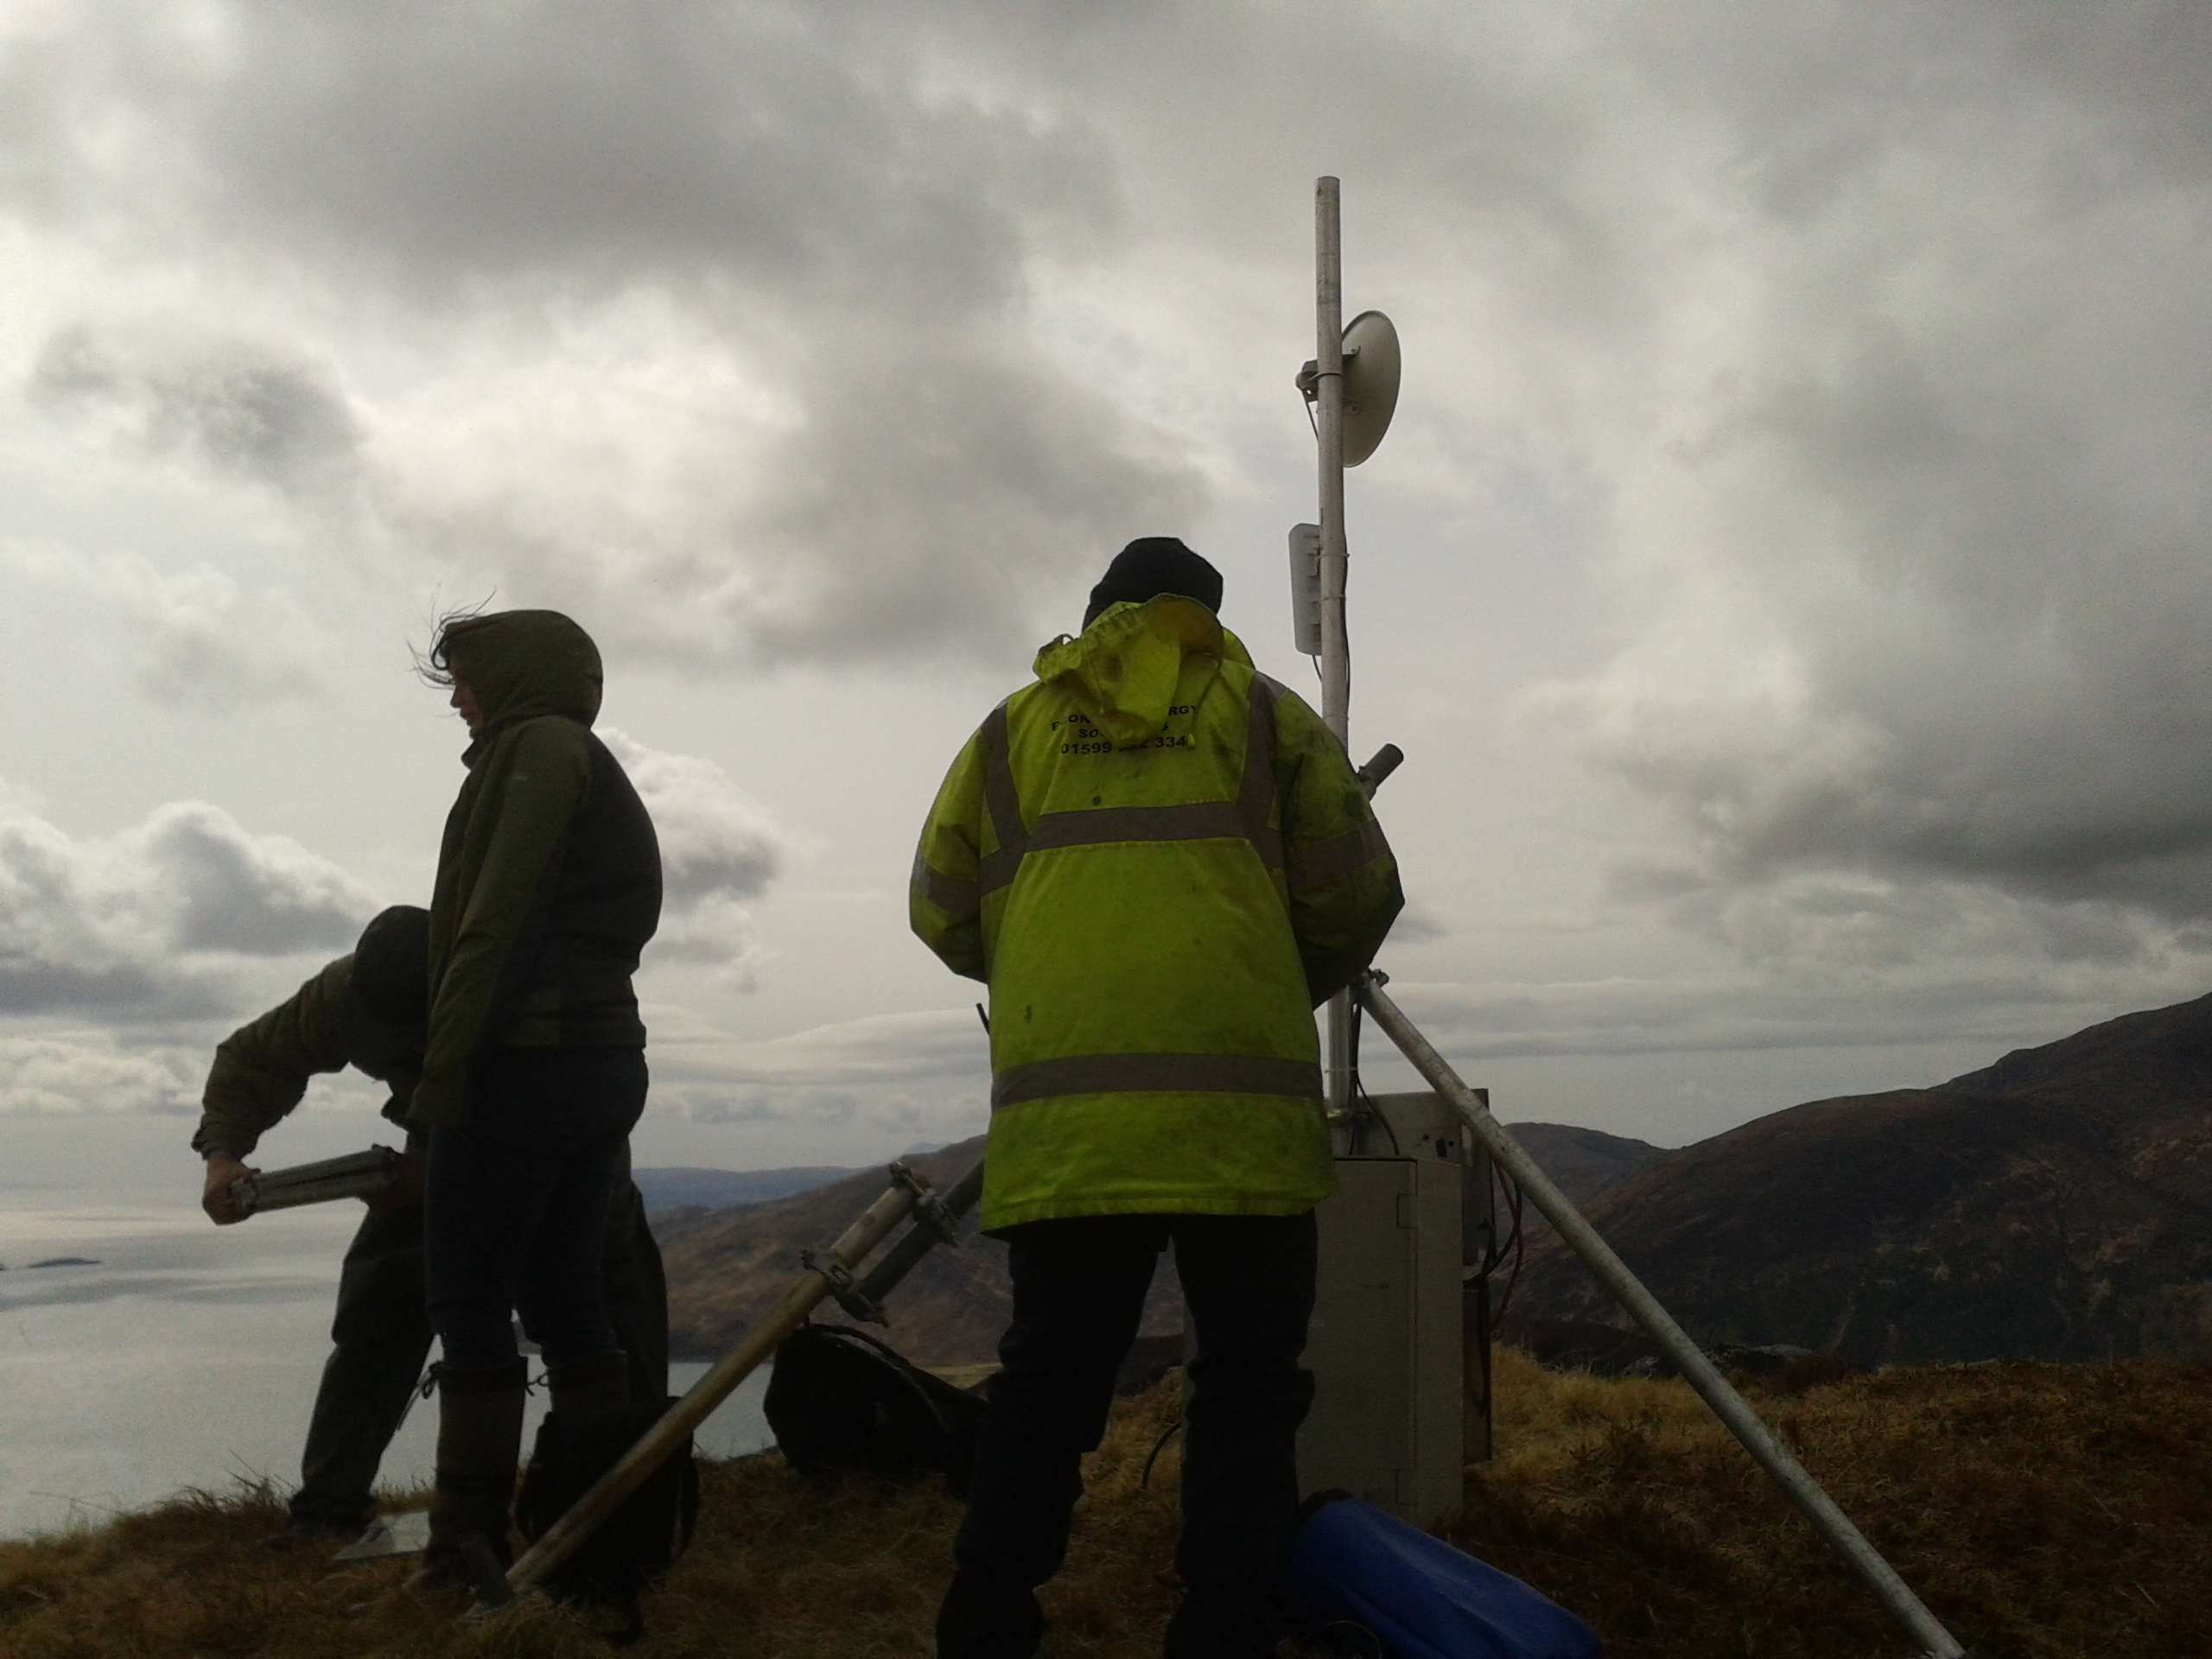
\includegraphics[height=1.1\paperheight]{glas_bheinn}
    };
  \end{tikzpicture}
\end{frame}
\begin{frame}
  \begin{tikzpicture}[overlay]
    \node at (5.5, -0.5) {%
      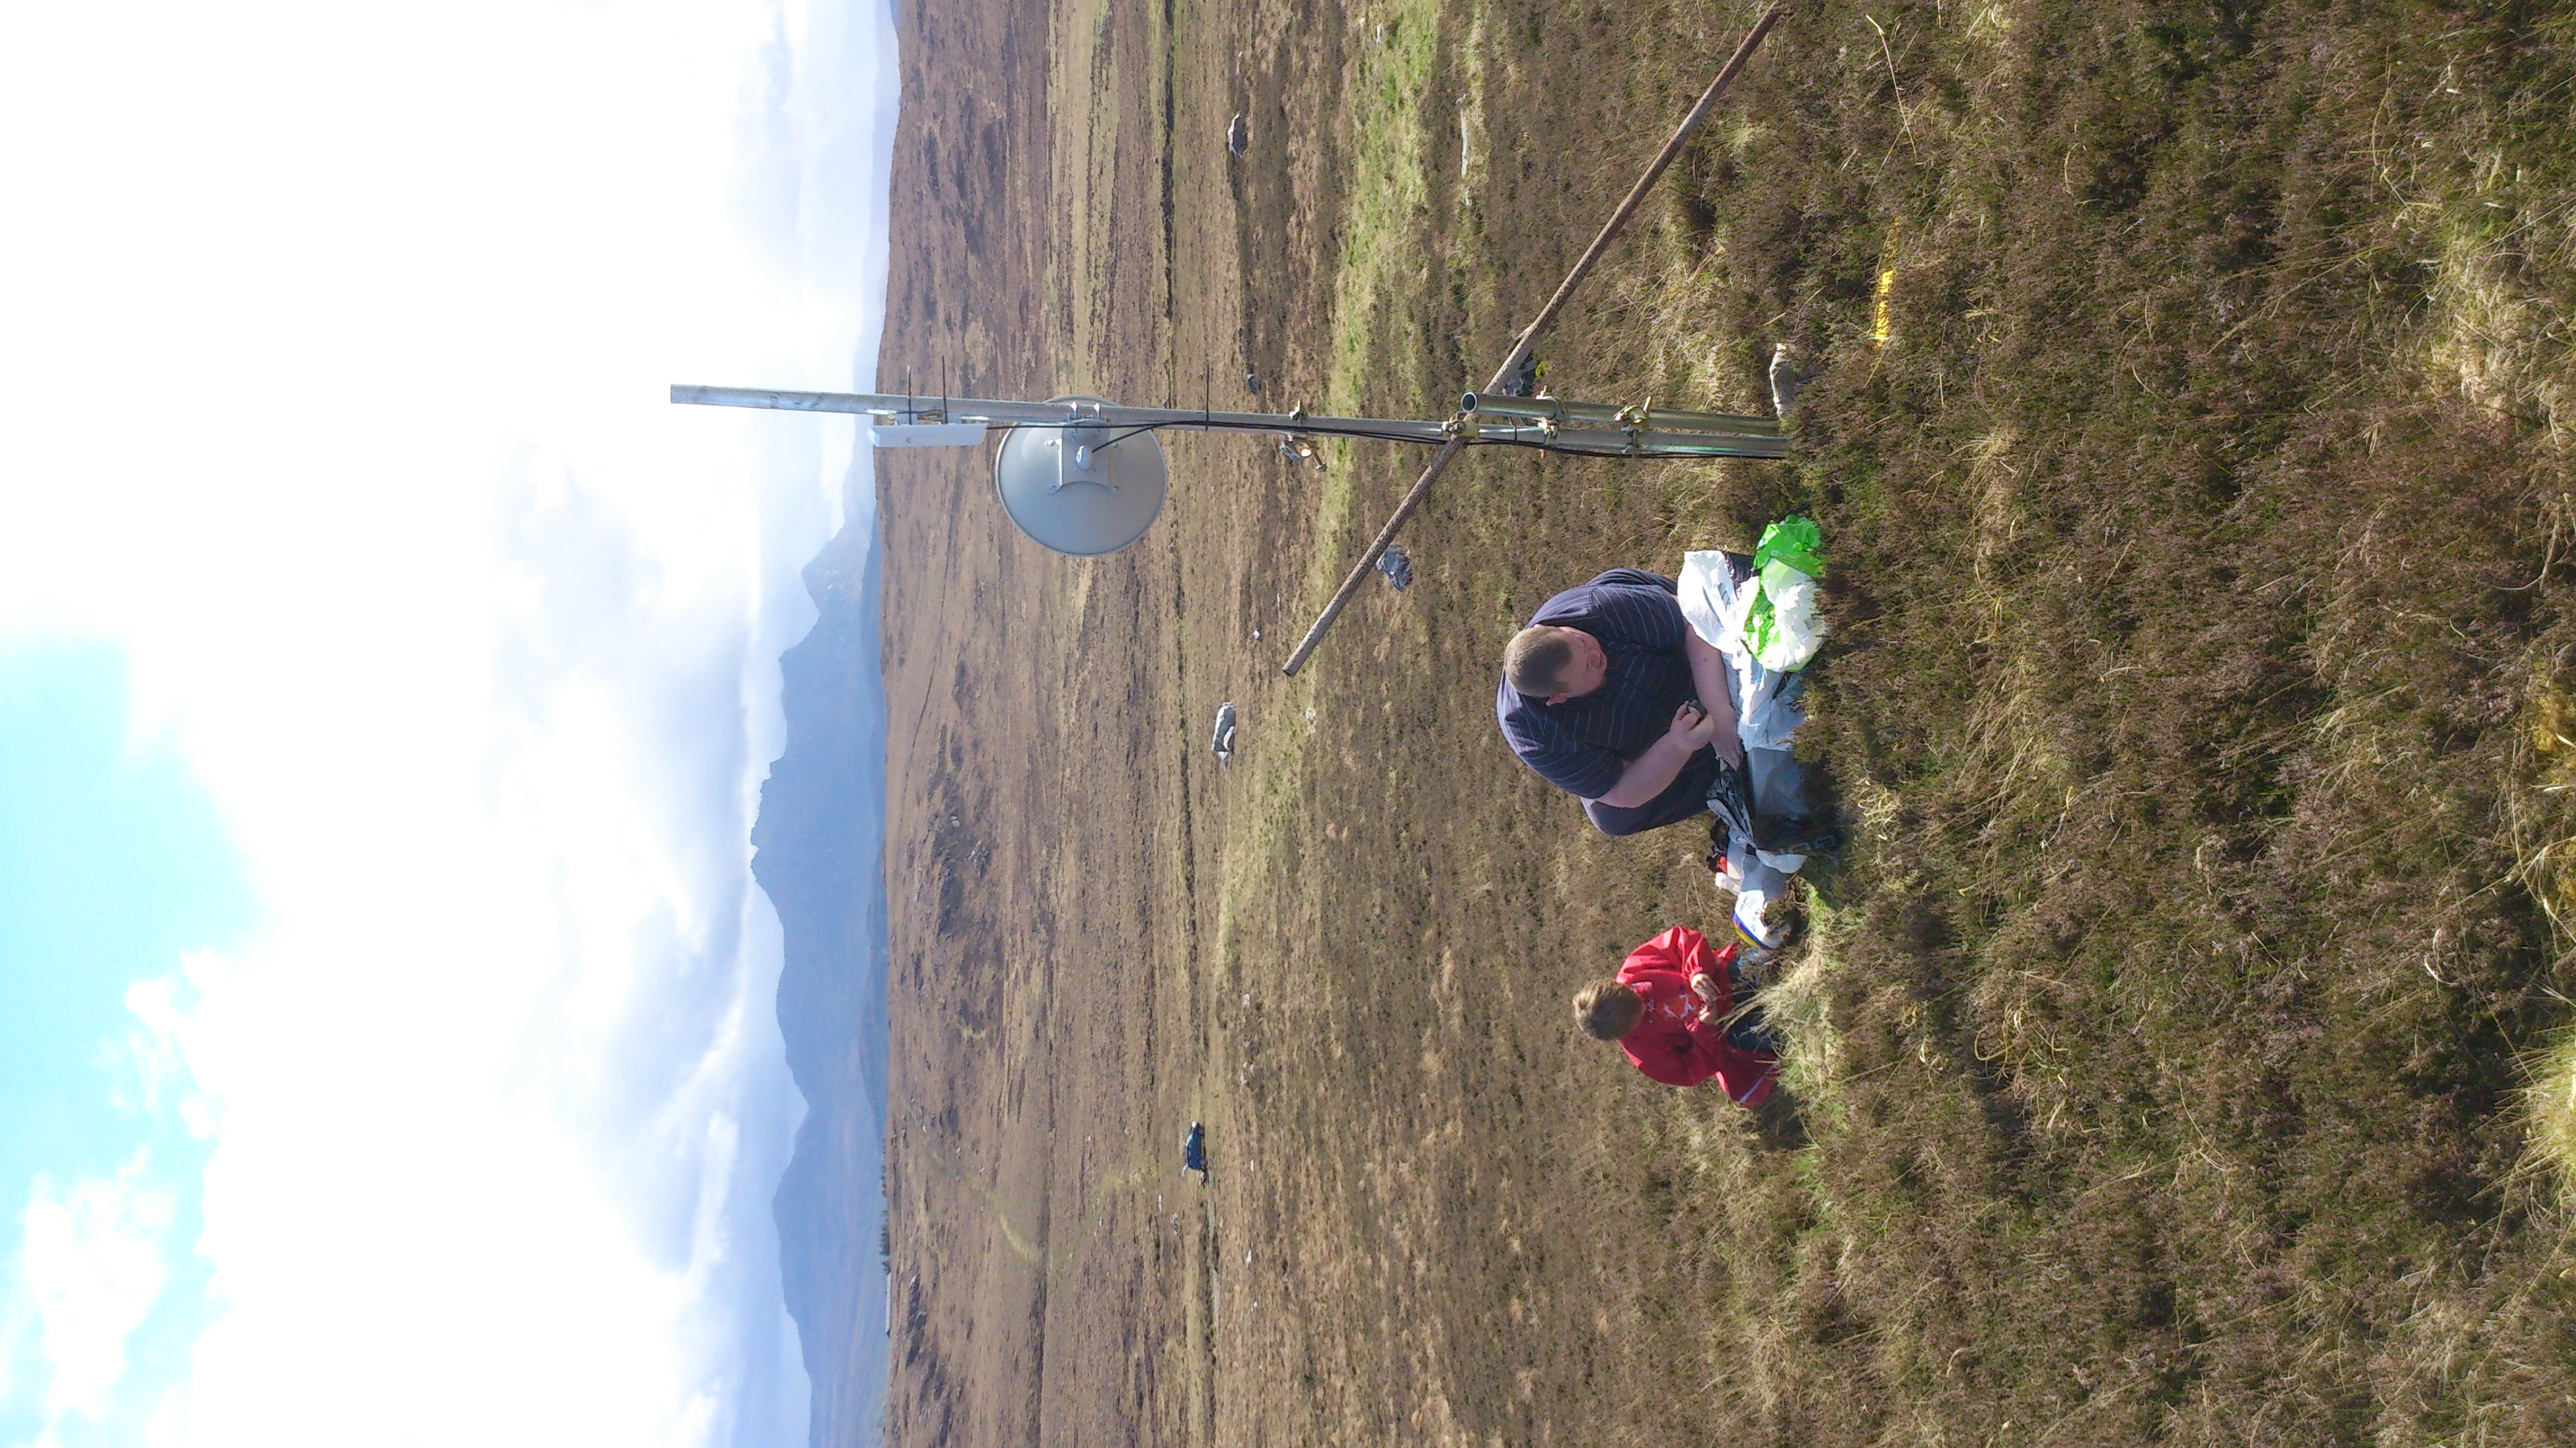
\includegraphics[width=1.1\paperwidth,angle=270]{melness}
    };
  \end{tikzpicture}
\end{frame}
\begin{frame}
  \begin{tikzpicture}[overlay]
    \node at (5.5, -0.5) {%
       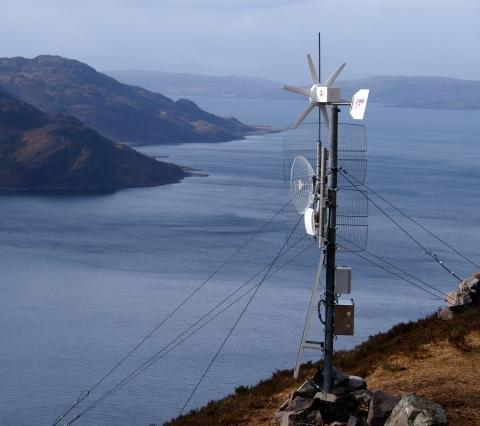
\includegraphics[width=1.05\paperwidth]{stick.jpg}
    };
    \end{tikzpicture}
\end{frame}
\begin{frame}
  \begin{tikzpicture}[overlay]
    \node at (5.5, -0.5) {%
      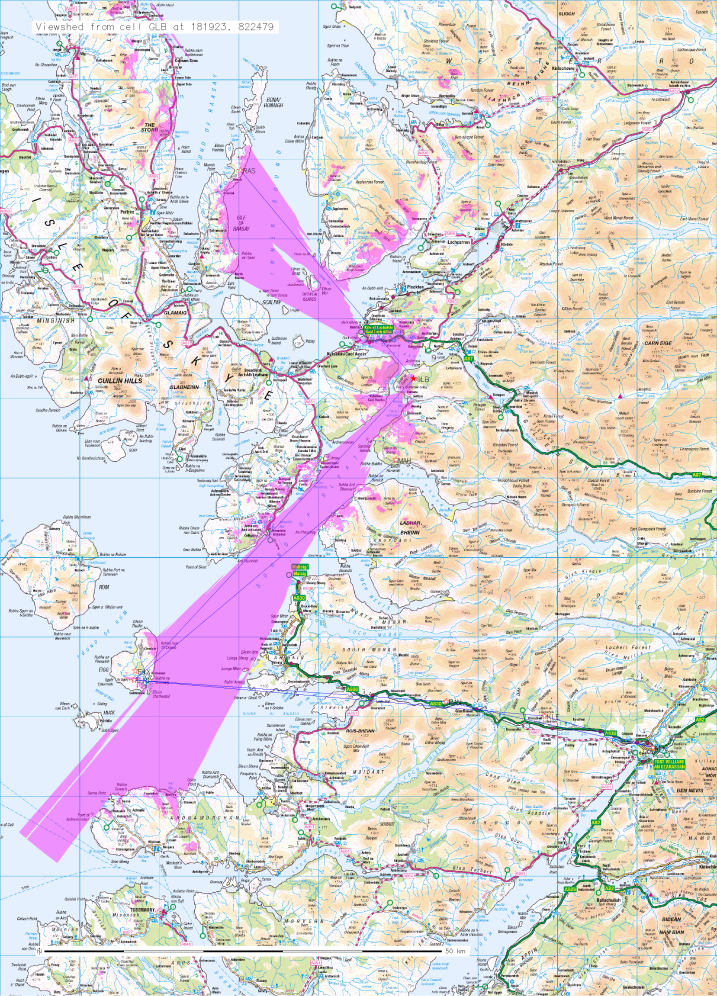
\includegraphics[height=1.1\paperheight]{GLB_viewshed}
    };
  \end{tikzpicture}
\end{frame}
\begin{frame}
  \begin{tikzpicture}[overlay]
    \node at (5.5, -0.5) {%
      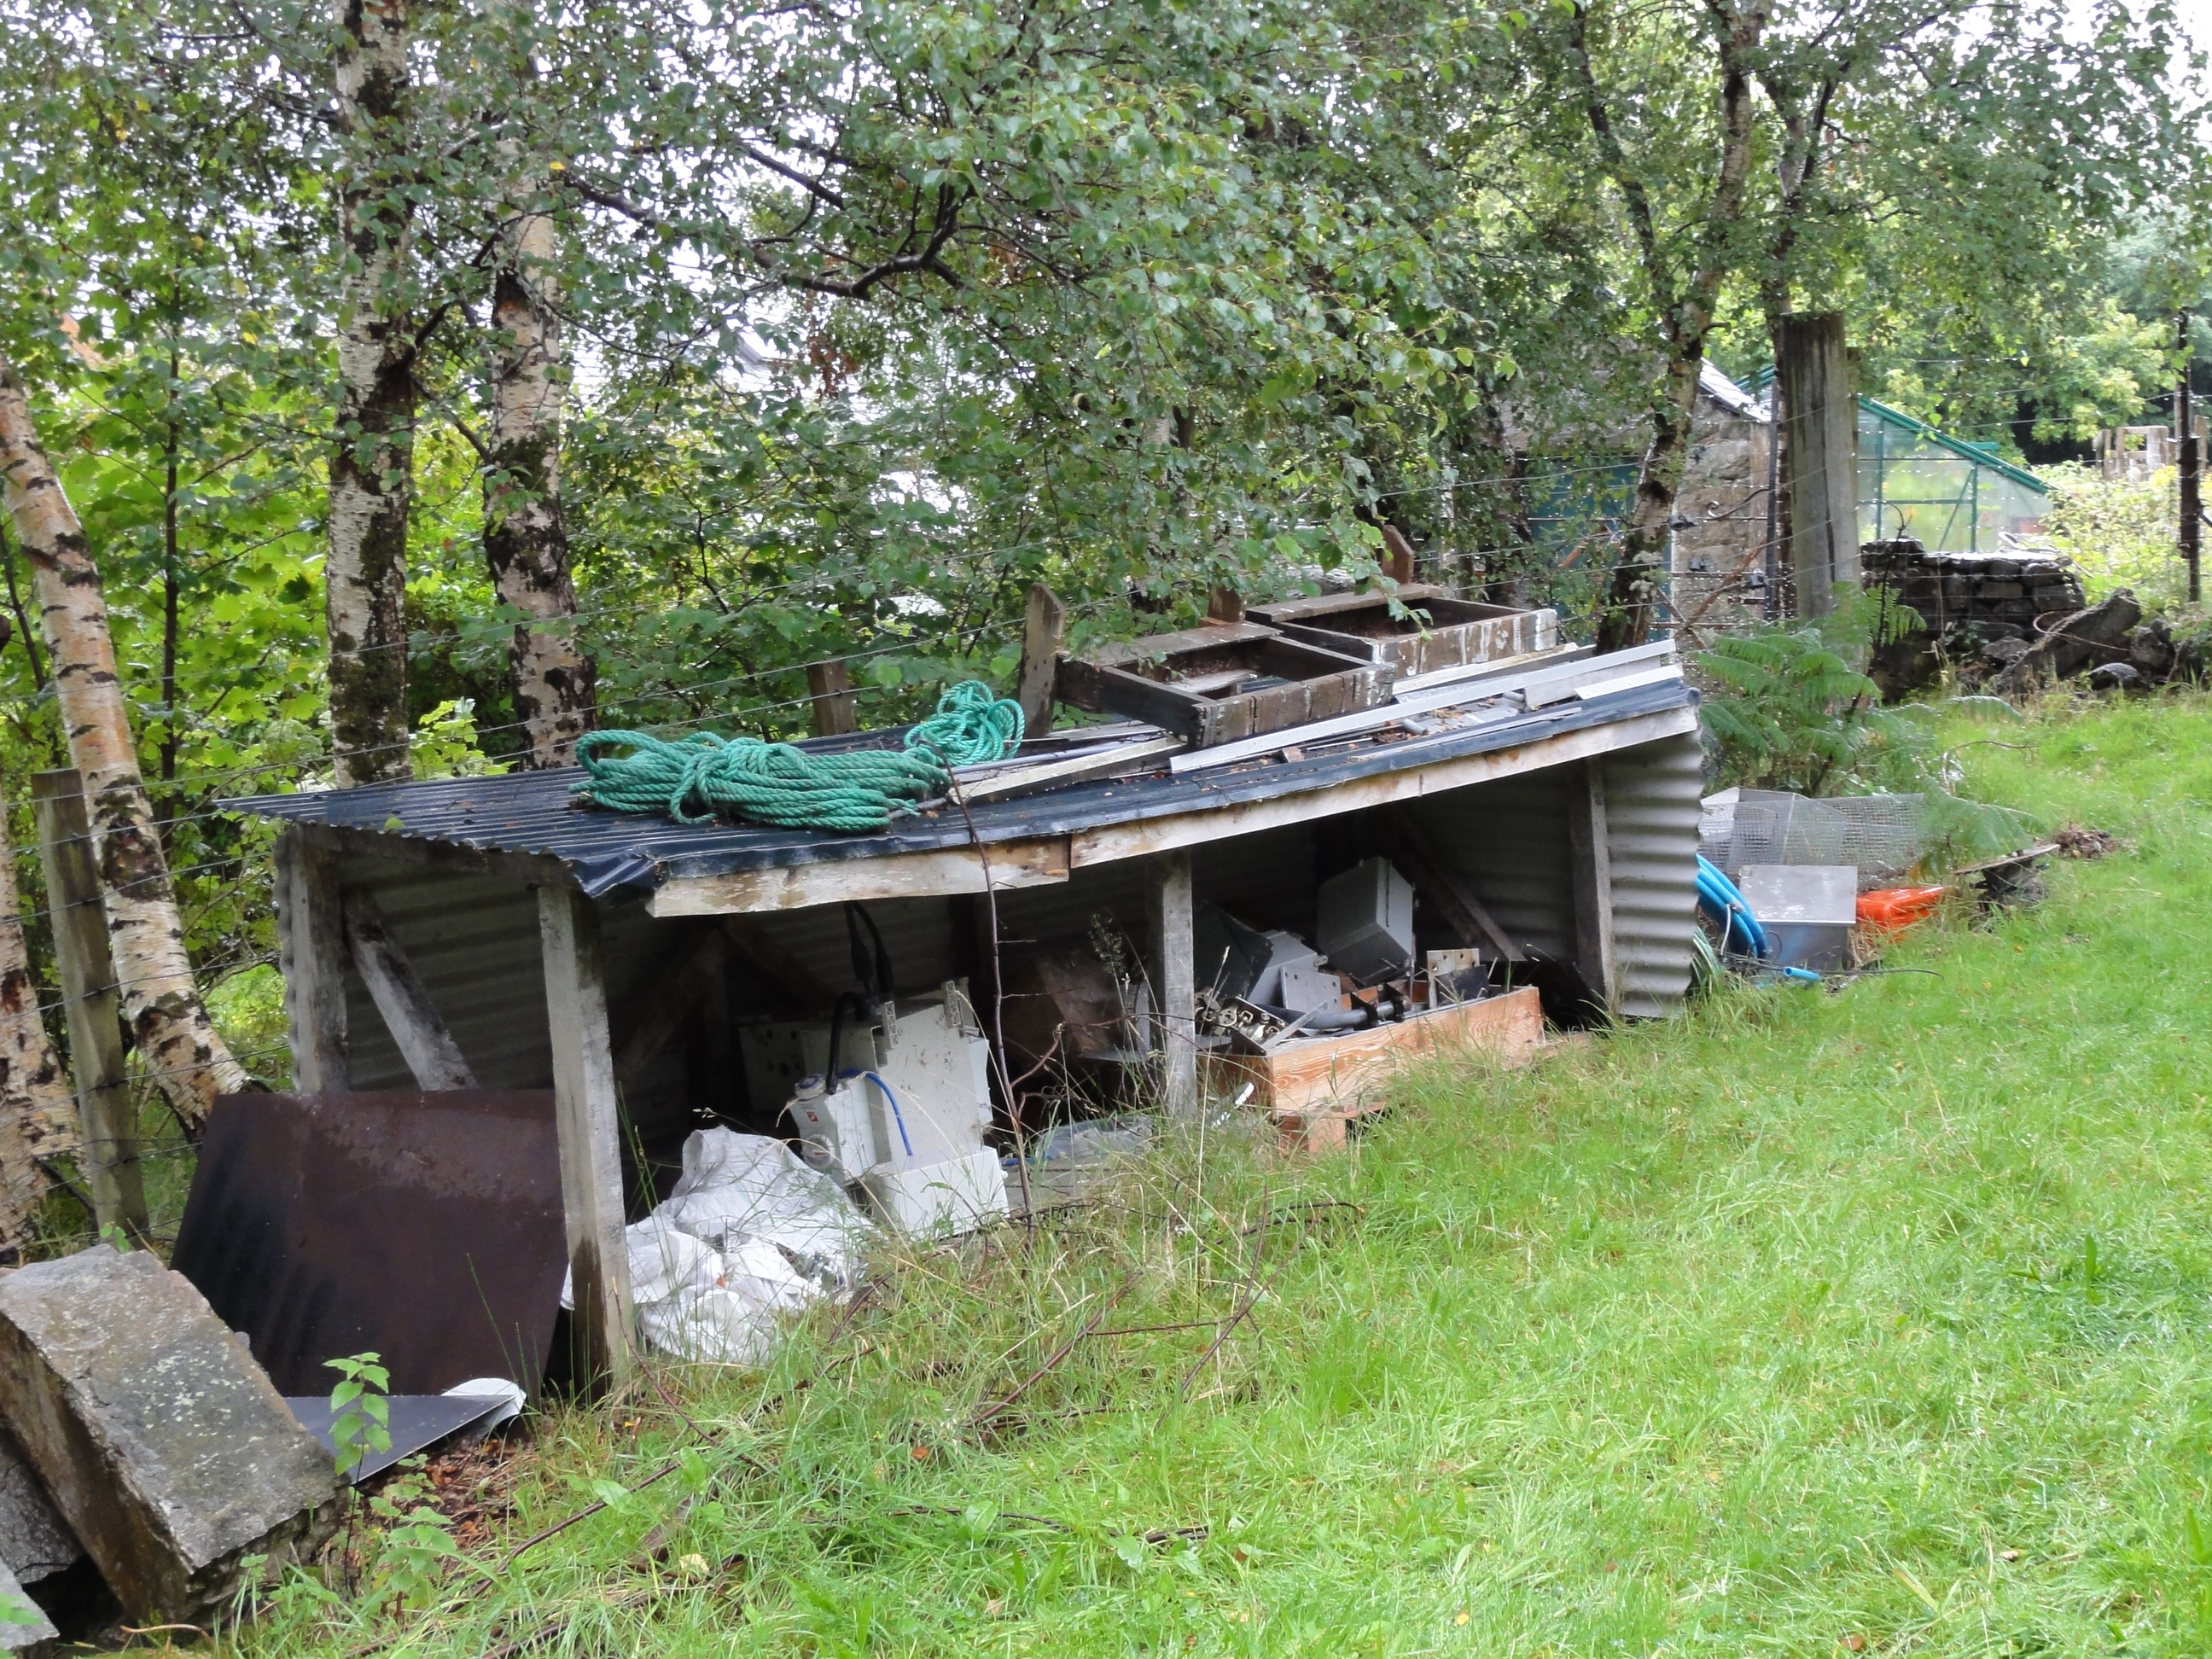
\includegraphics[width=1.07\paperwidth]{junkpile.jpg}
    };
    \end{tikzpicture}
\end{frame}
\begin{frame}
  \begin{tikzpicture}[overlay]
    \node at (5.5, -0.5) {%
      \includegraphics[width=1.07\paperwidth]{corran-testing.jpg}
    };
    \end{tikzpicture}
\end{frame}
\begin{frame}
  \begin{tikzpicture}[overlay]
    \node at (5.5, -0.5) {%
      \includegraphics[height=1.1\paperheight]{inver-mast.jpg}
    };
    \end{tikzpicture}
\end{frame}
%\begin{frame}
%  \begin{tikzpicture}[overlay]
%    \node at (5.5, -0.5) {%
%      \includegraphics[width=1.1\paperwidth]{creagan-dearga-mast.jpg}
%    };
%  \end{tikzpicture}
%\end{frame}
\begin{frame}
  \begin{tikzpicture}[overlay]
    \node at (5.5, -0.5) {%
      \includegraphics[width=1.07\paperwidth]{mhialairigh-from-behind.jpg}
    };
    \end{tikzpicture}
\end{frame}
\begin{frame}
  \begin{tikzpicture}[overlay]
    \node at (5, 1) {%
      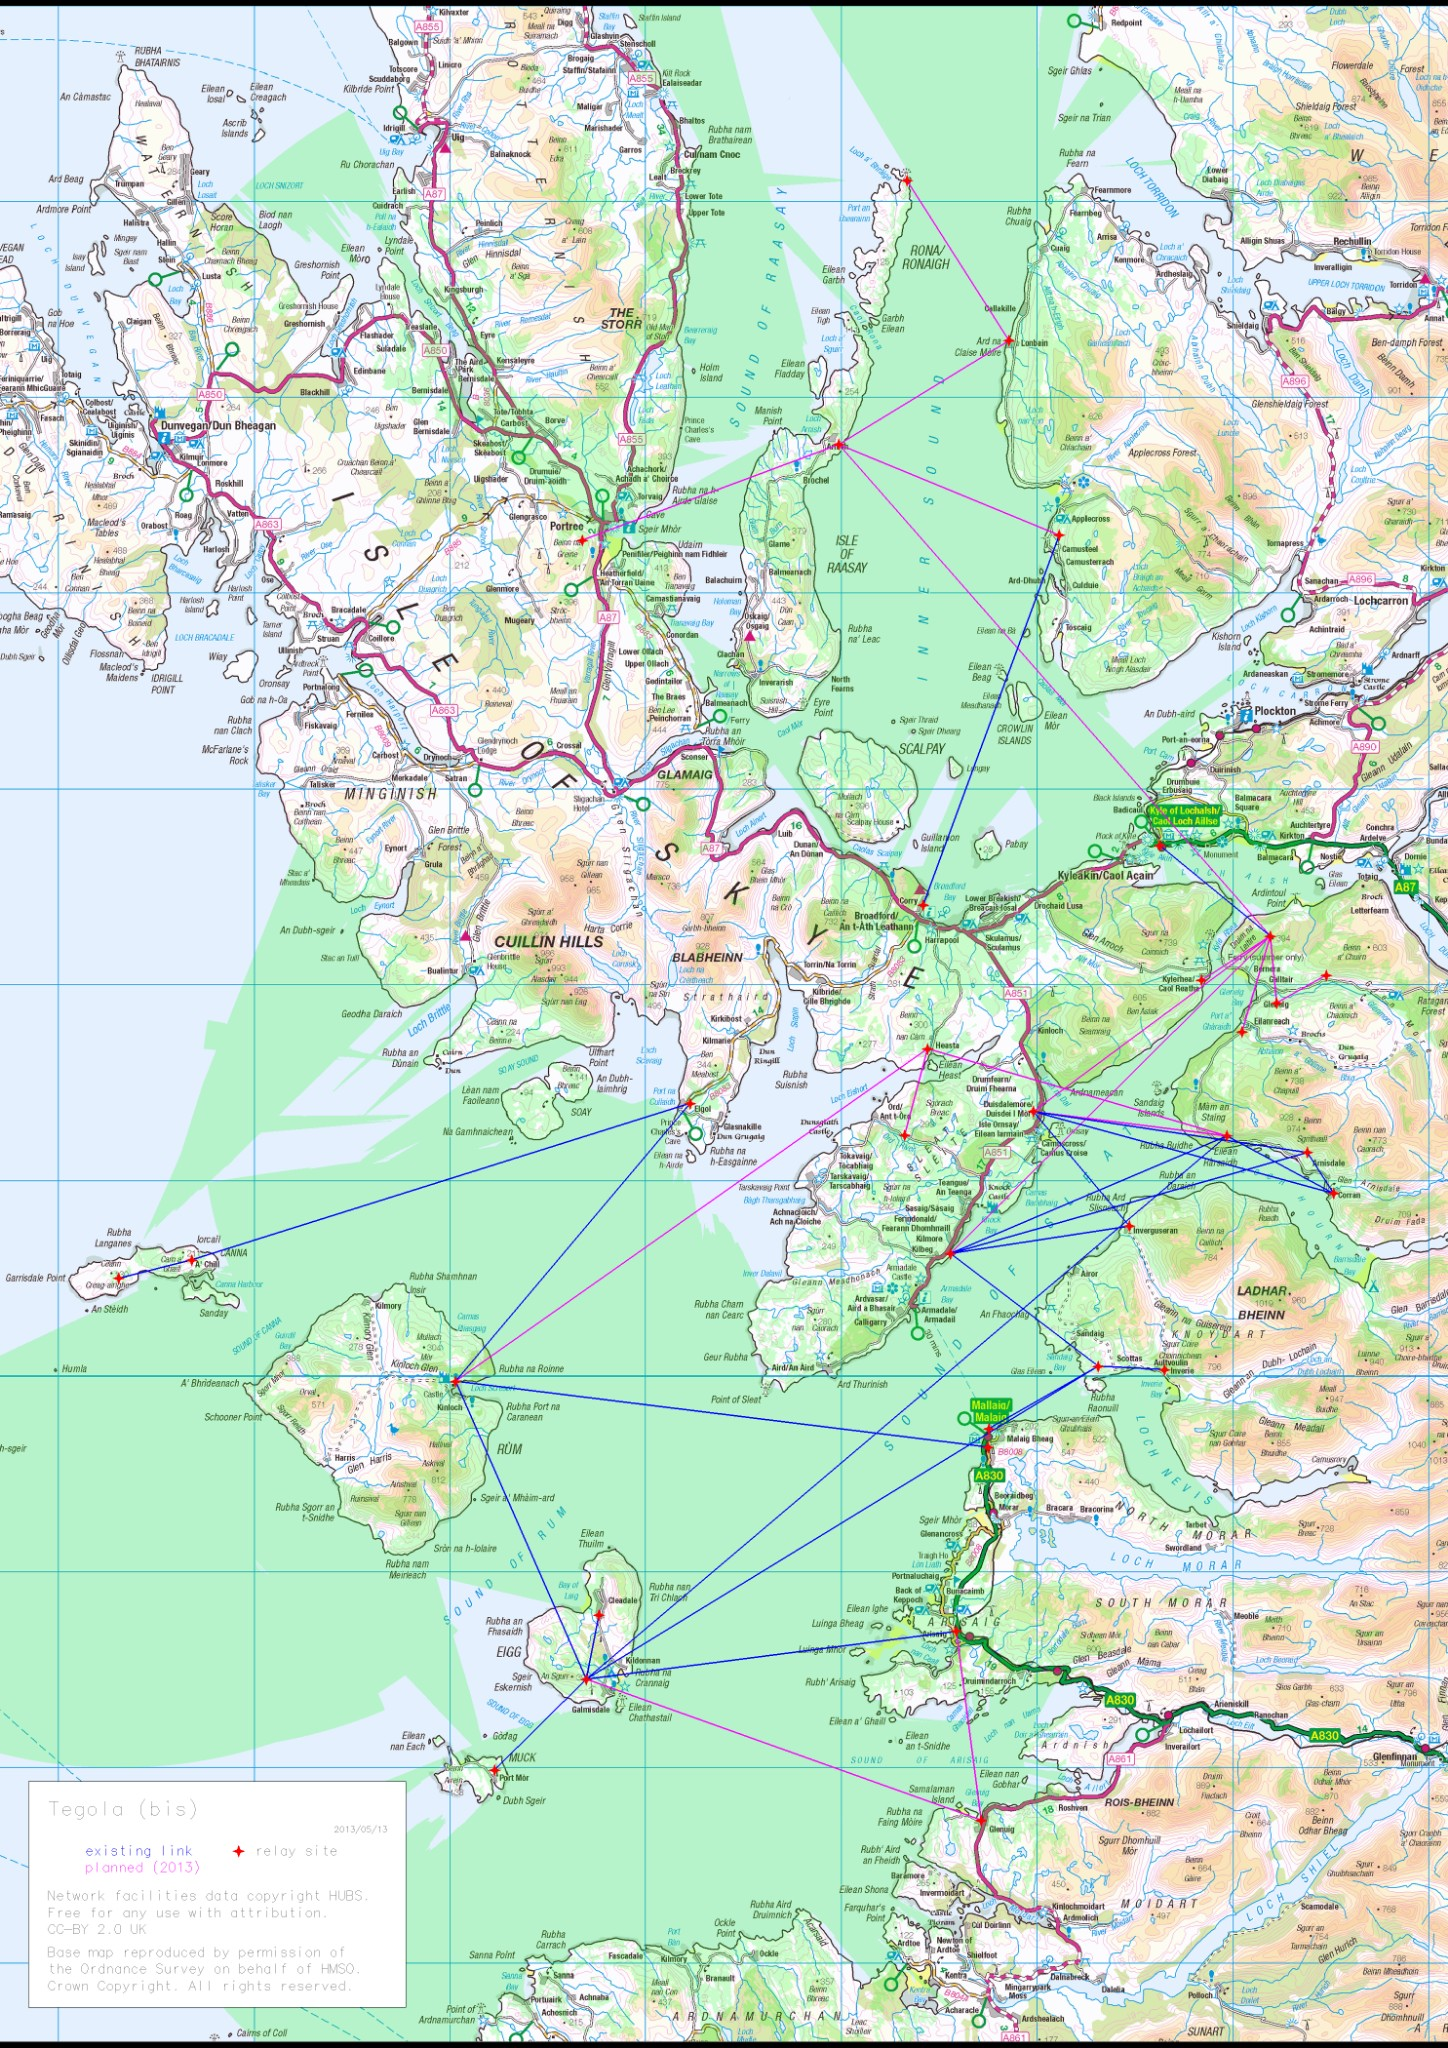
\includegraphics[width=1.05\paperwidth]{west_coast_a4.jpg}
    };
  \end{tikzpicture}
\end{frame}
\begin{frame}
  \begin{tikzpicture}[overlay]
    \node at (5.5, -0.5) {%
      \includegraphics[width=0.8\paperwidth]{west-coast-detail}
    };
  \end{tikzpicture}
\end{frame}
\begin{frame}
  \begin{tikzpicture}[overlay]
    \node at (5.5, -0.5) {%
      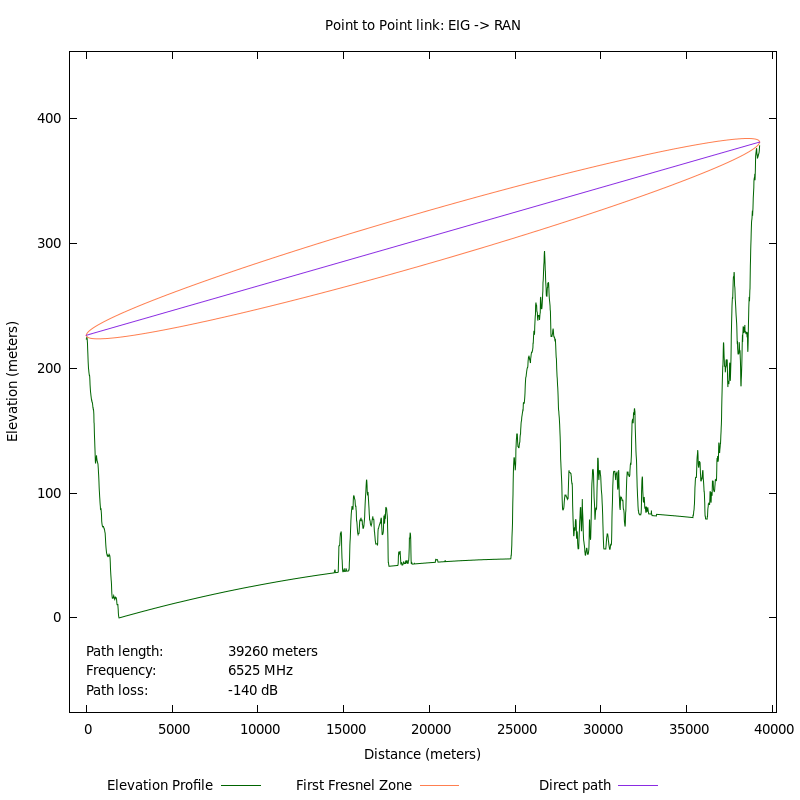
\includegraphics[width=0.7\paperwidth]{EIG_RAN.png}
    };
  \end{tikzpicture}
\end{frame}
\begin{frame}
  \begin{tikzpicture}[overlay]
    \node at (5.5, -0.5) {%
      \includegraphics[height=\paperheight]{tommy-diversity.jpg}
    };
  \end{tikzpicture}
\end{frame}
\begin{frame}
  \begin{tikzpicture}[overlay]
    \node at (5.5, -0.5) {%
      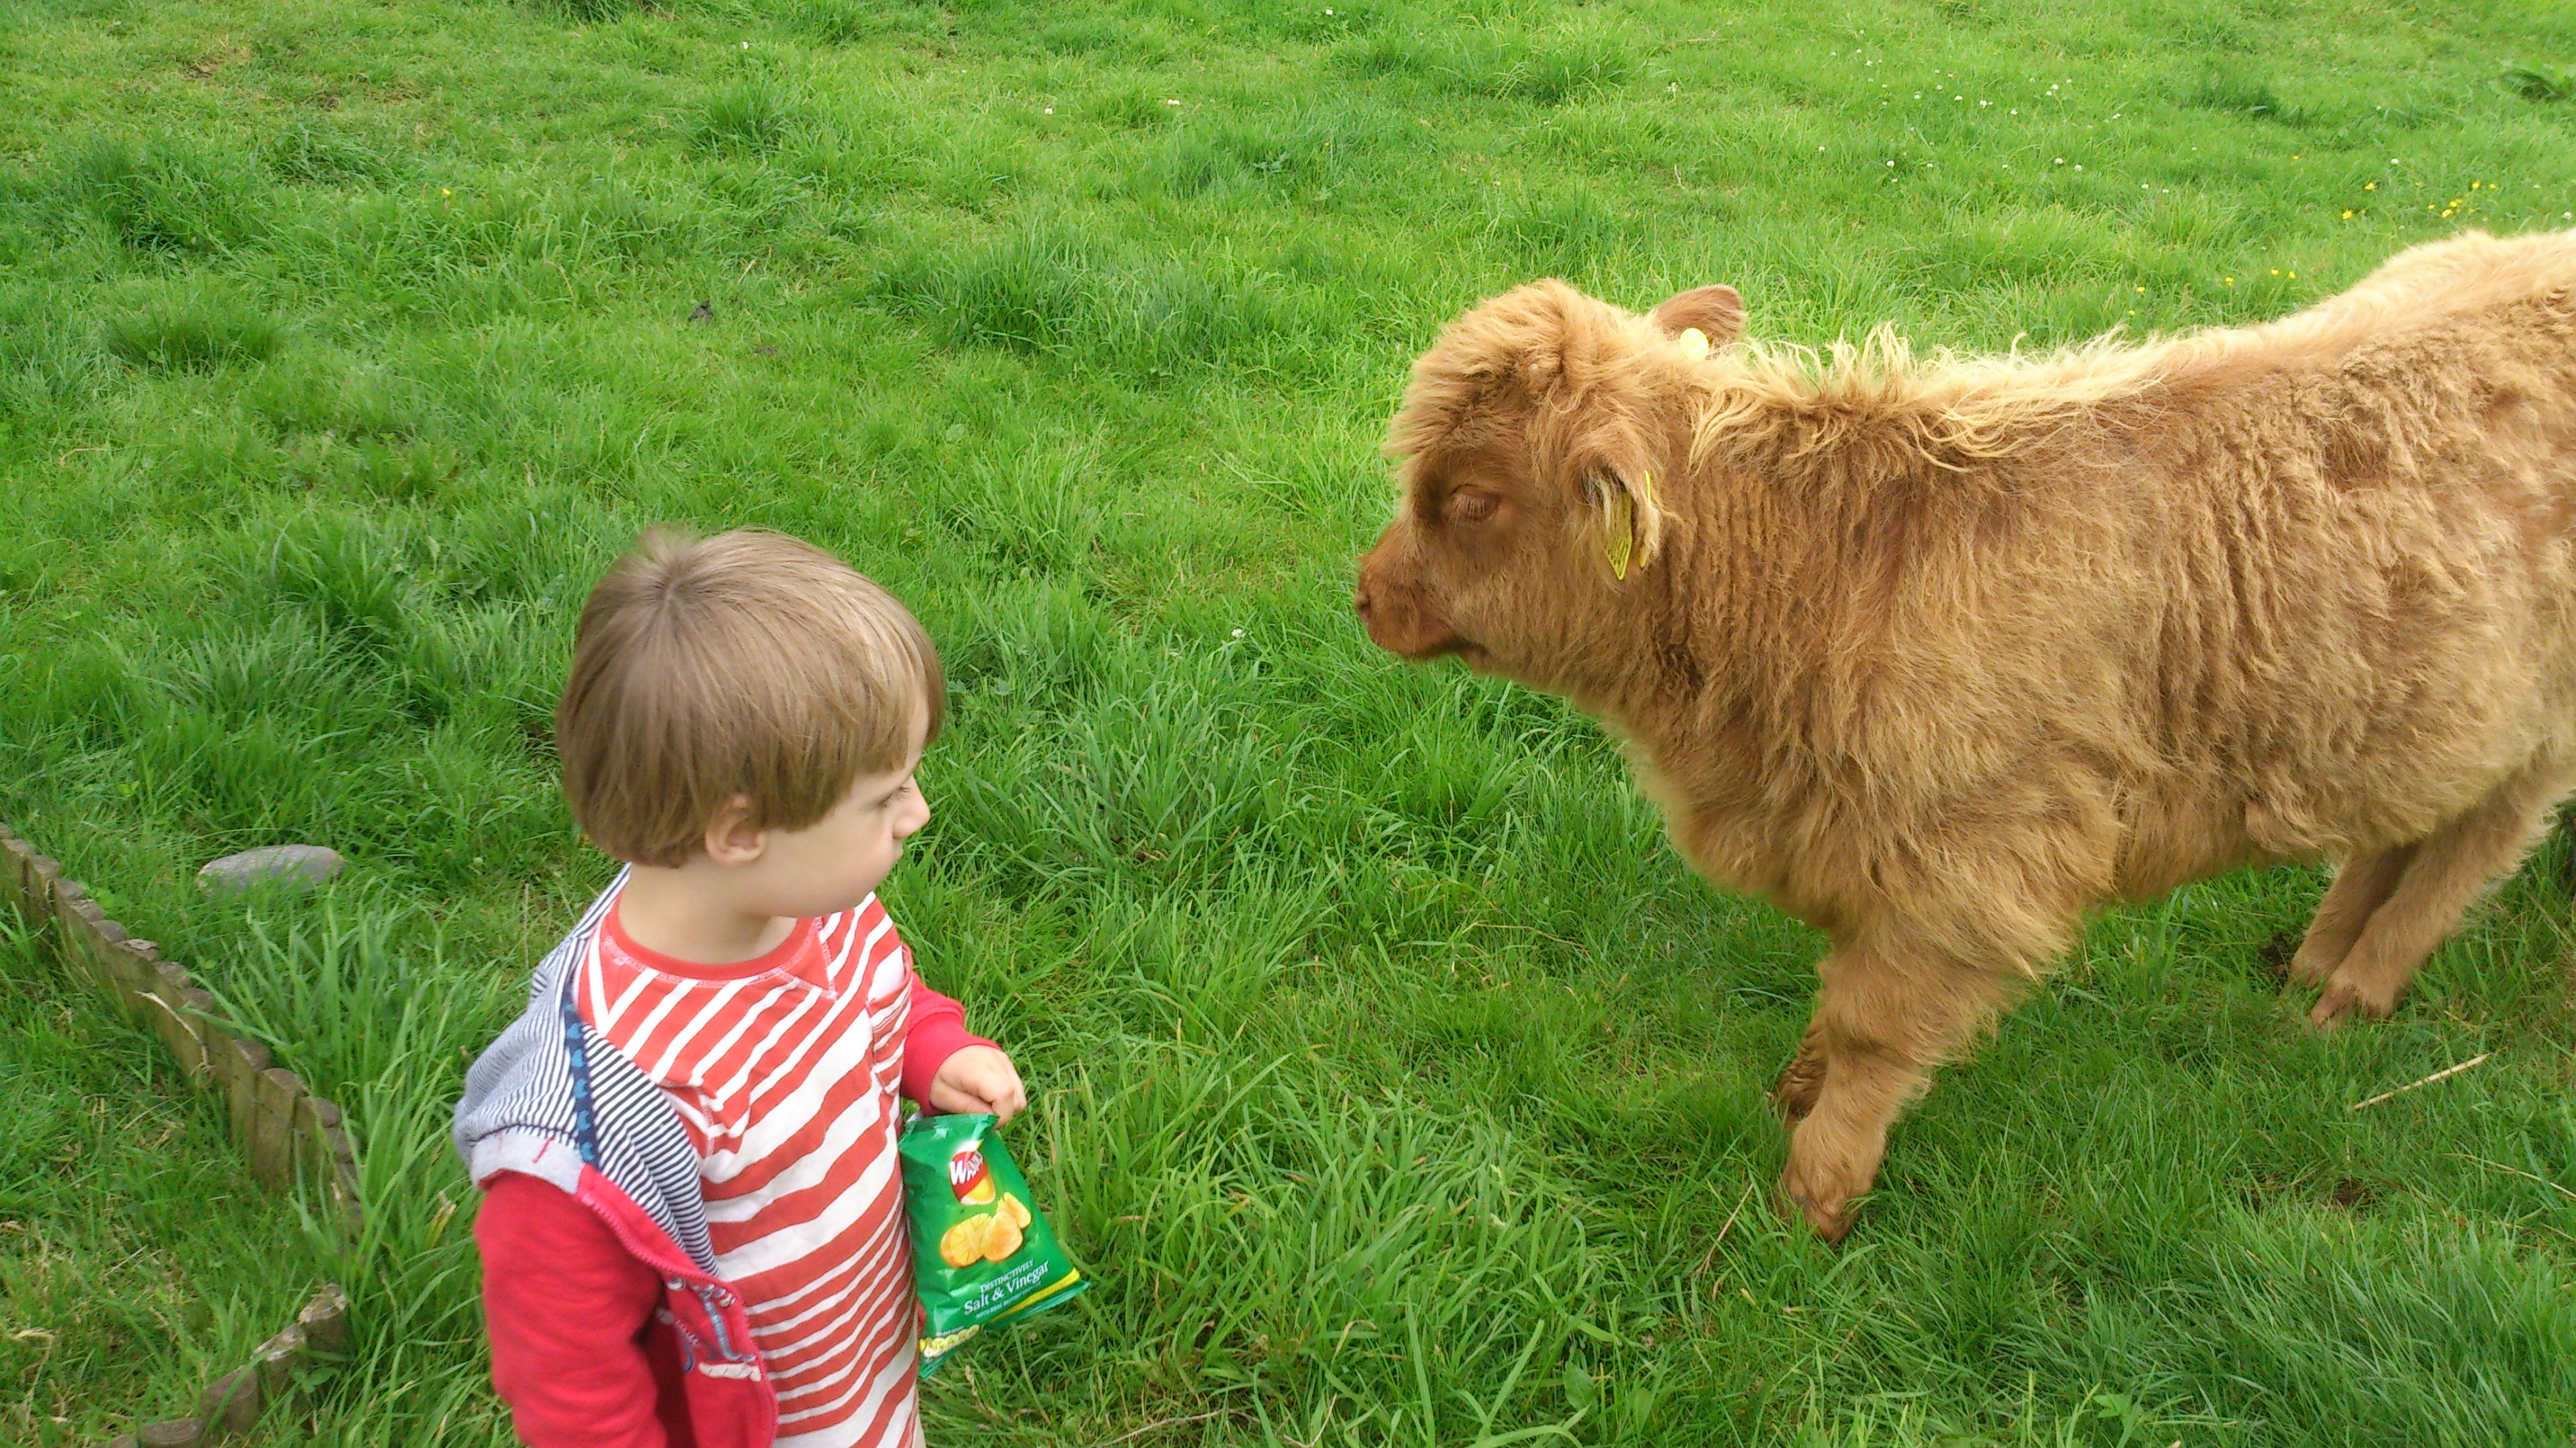
\includegraphics[height=1.1\paperheight]{cow_hazard}
    };
  \end{tikzpicture}
\end{frame}
\begin{frame}
  \begin{tikzpicture}[overlay]
    \node at (5.5, -0.5) {%
      \includegraphics[width=1.1\paperwidth]{portree-3d.png}
    };
  \end{tikzpicture}
\end{frame}
\begin{frame}
  \begin{tikzpicture}[overlay]
    \node at (5.5, -0.5) {%
      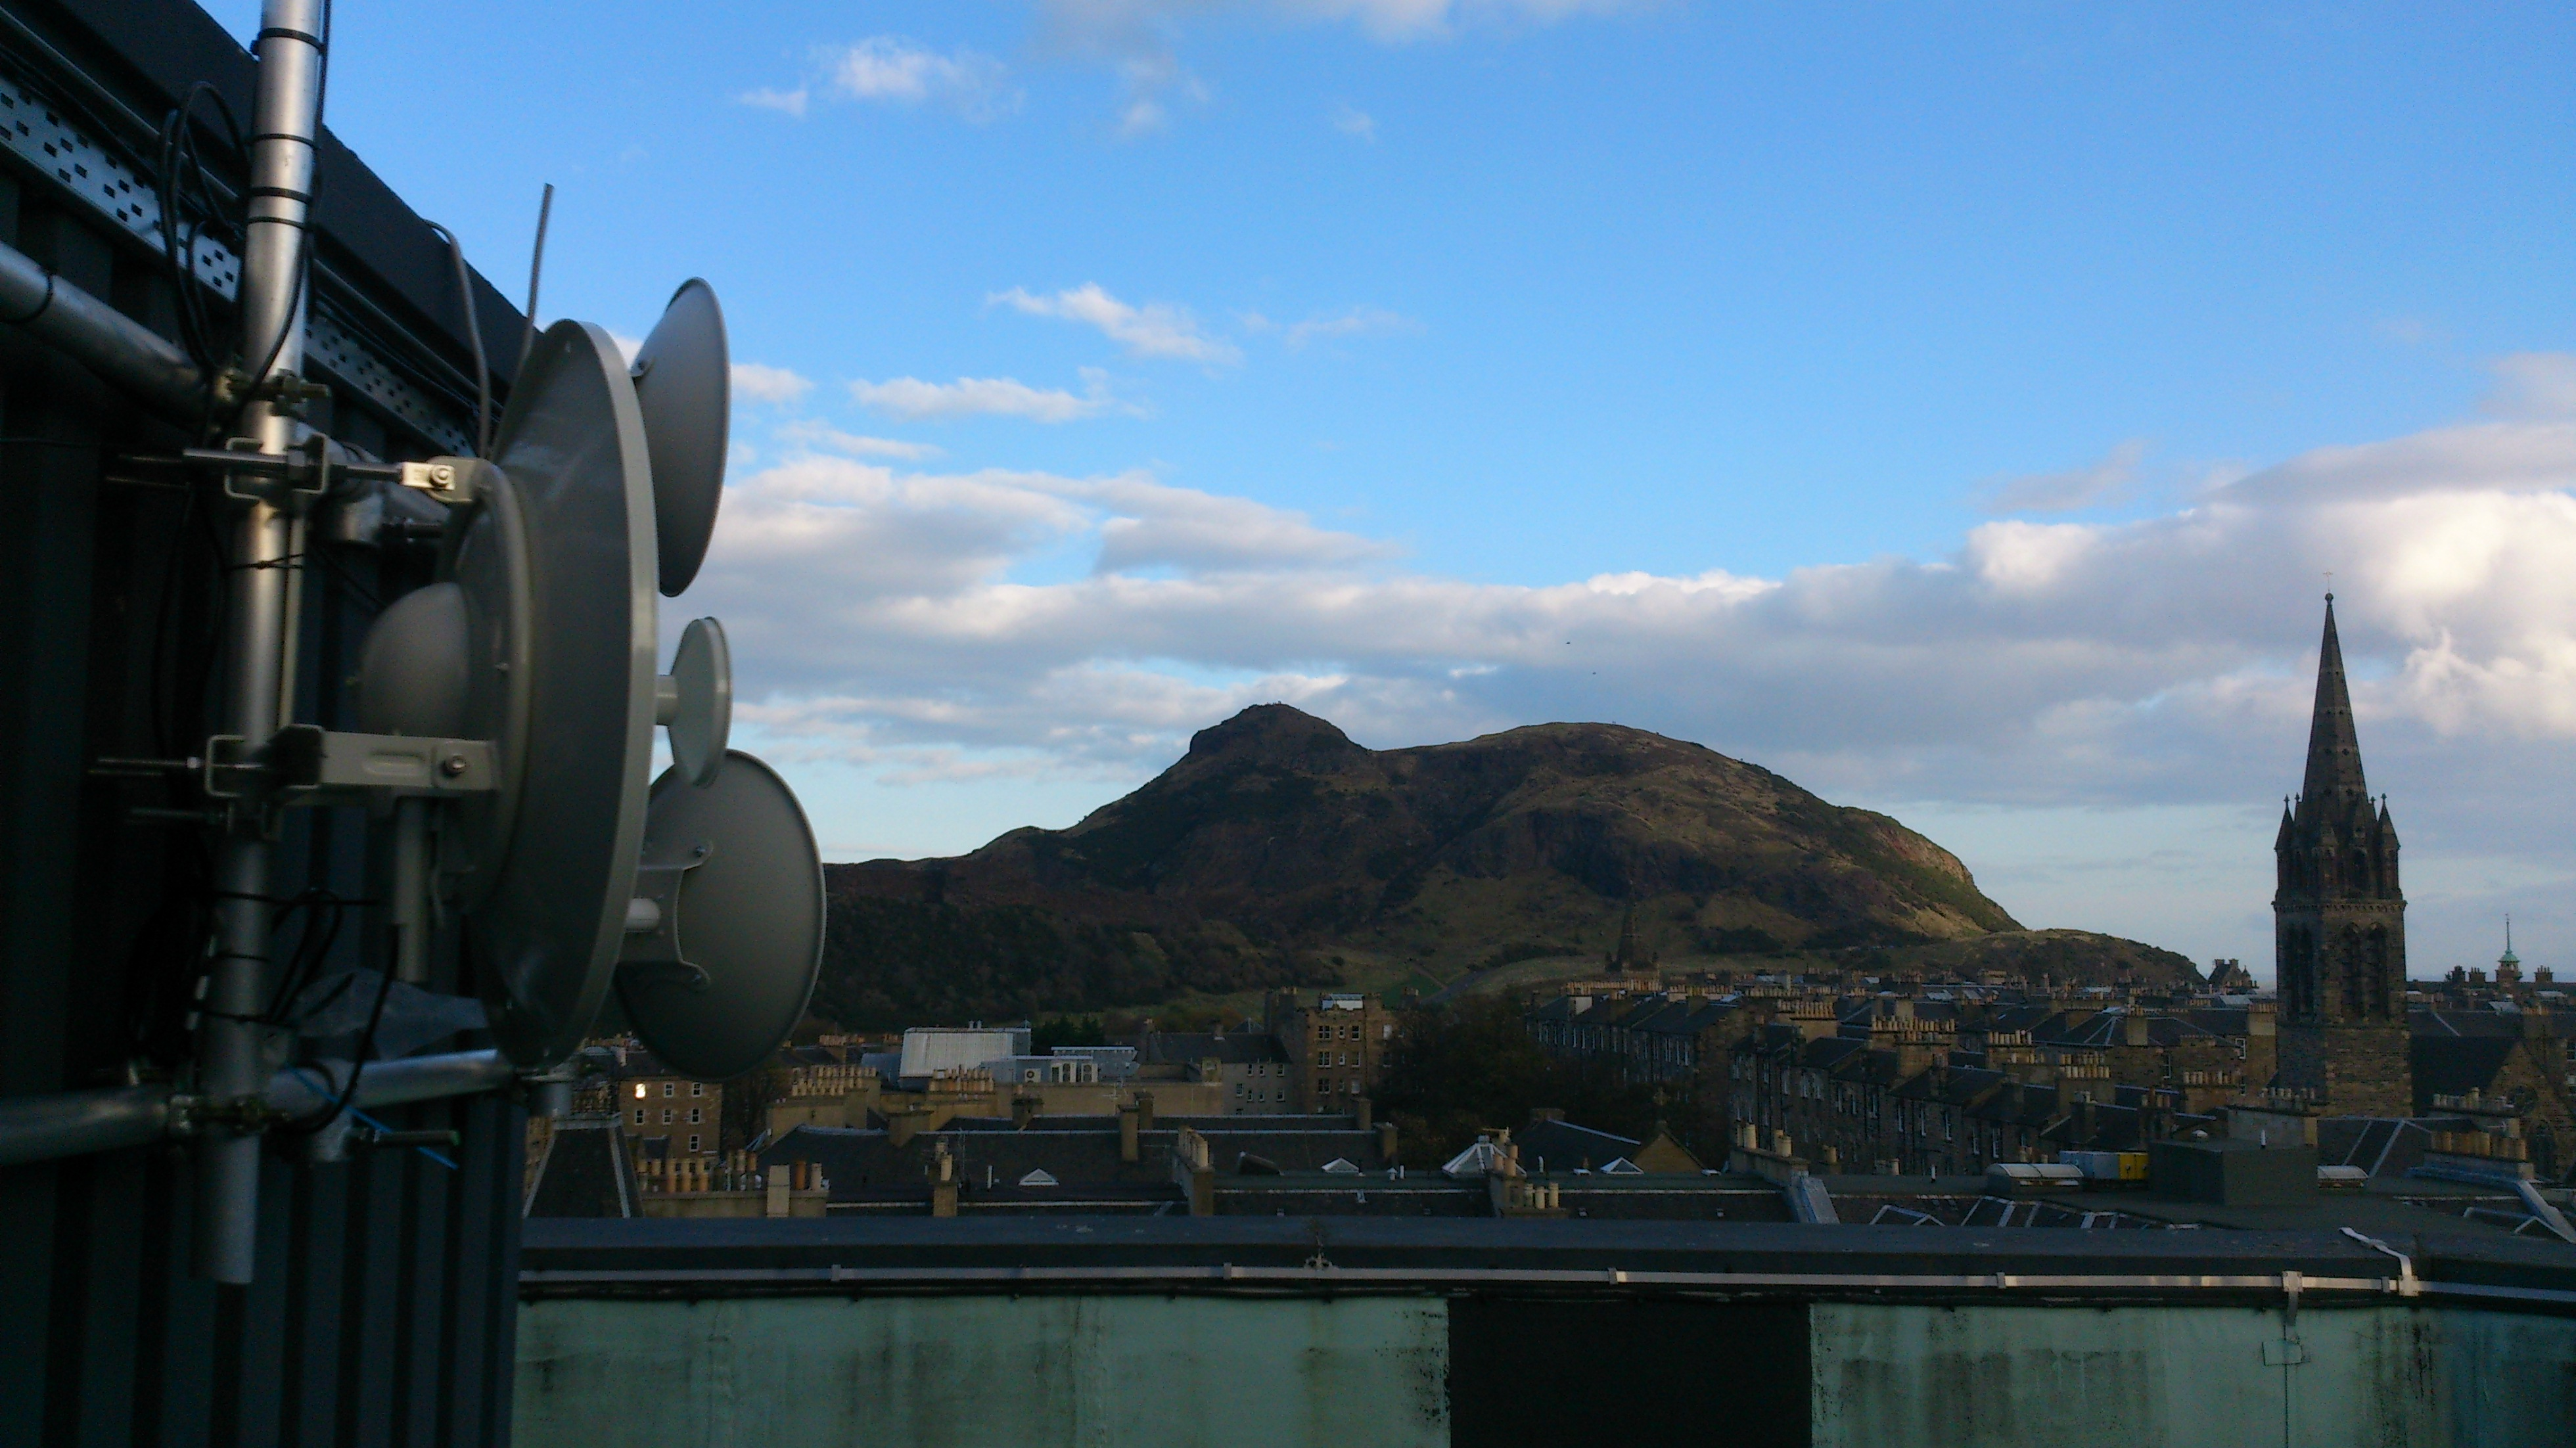
\includegraphics[height=1.1\paperheight]{tc_south}
    };
  \end{tikzpicture}
\end{frame}
\begin{frame}
  \begin{tikzpicture}[overlay]
    \node at (5.5, -0.5) {%
      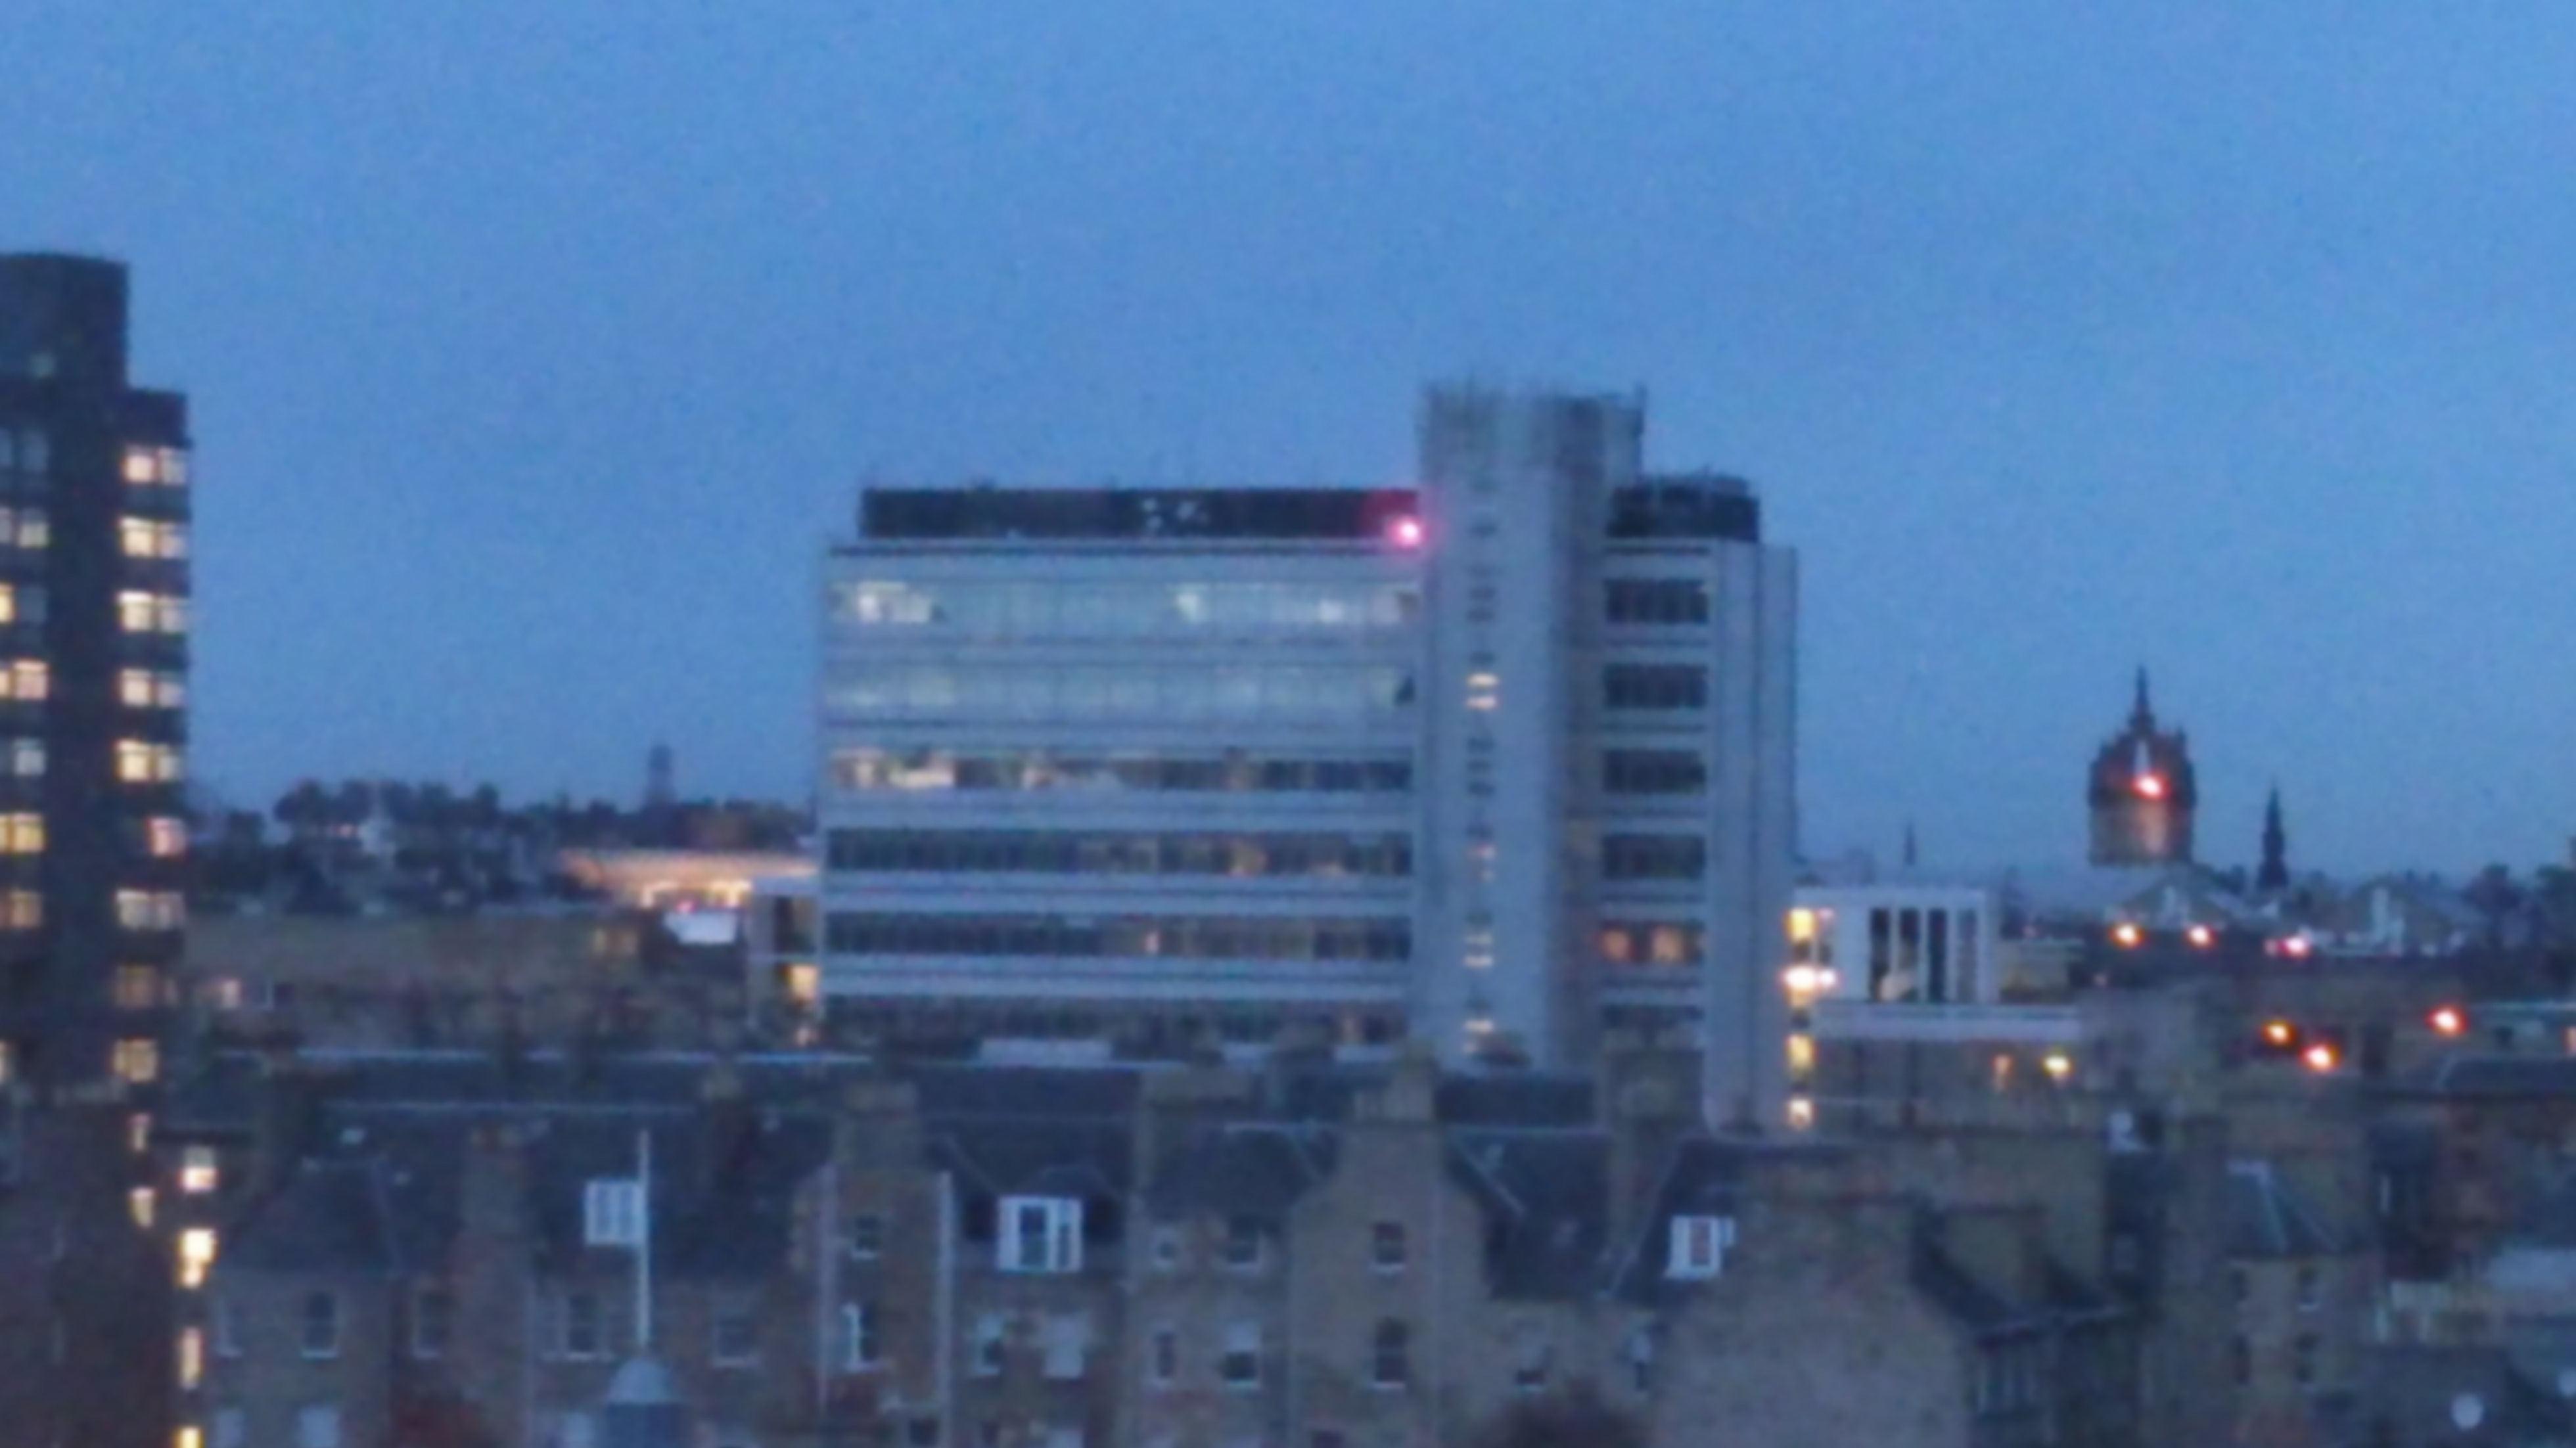
\includegraphics[height=1.1\paperheight]{at_laser}
    };
  \end{tikzpicture}
\end{frame}
% \begin{frame}
%   \begin{tikzpicture}[overlay]
%     \node at (5.5, -0.5) {%
%       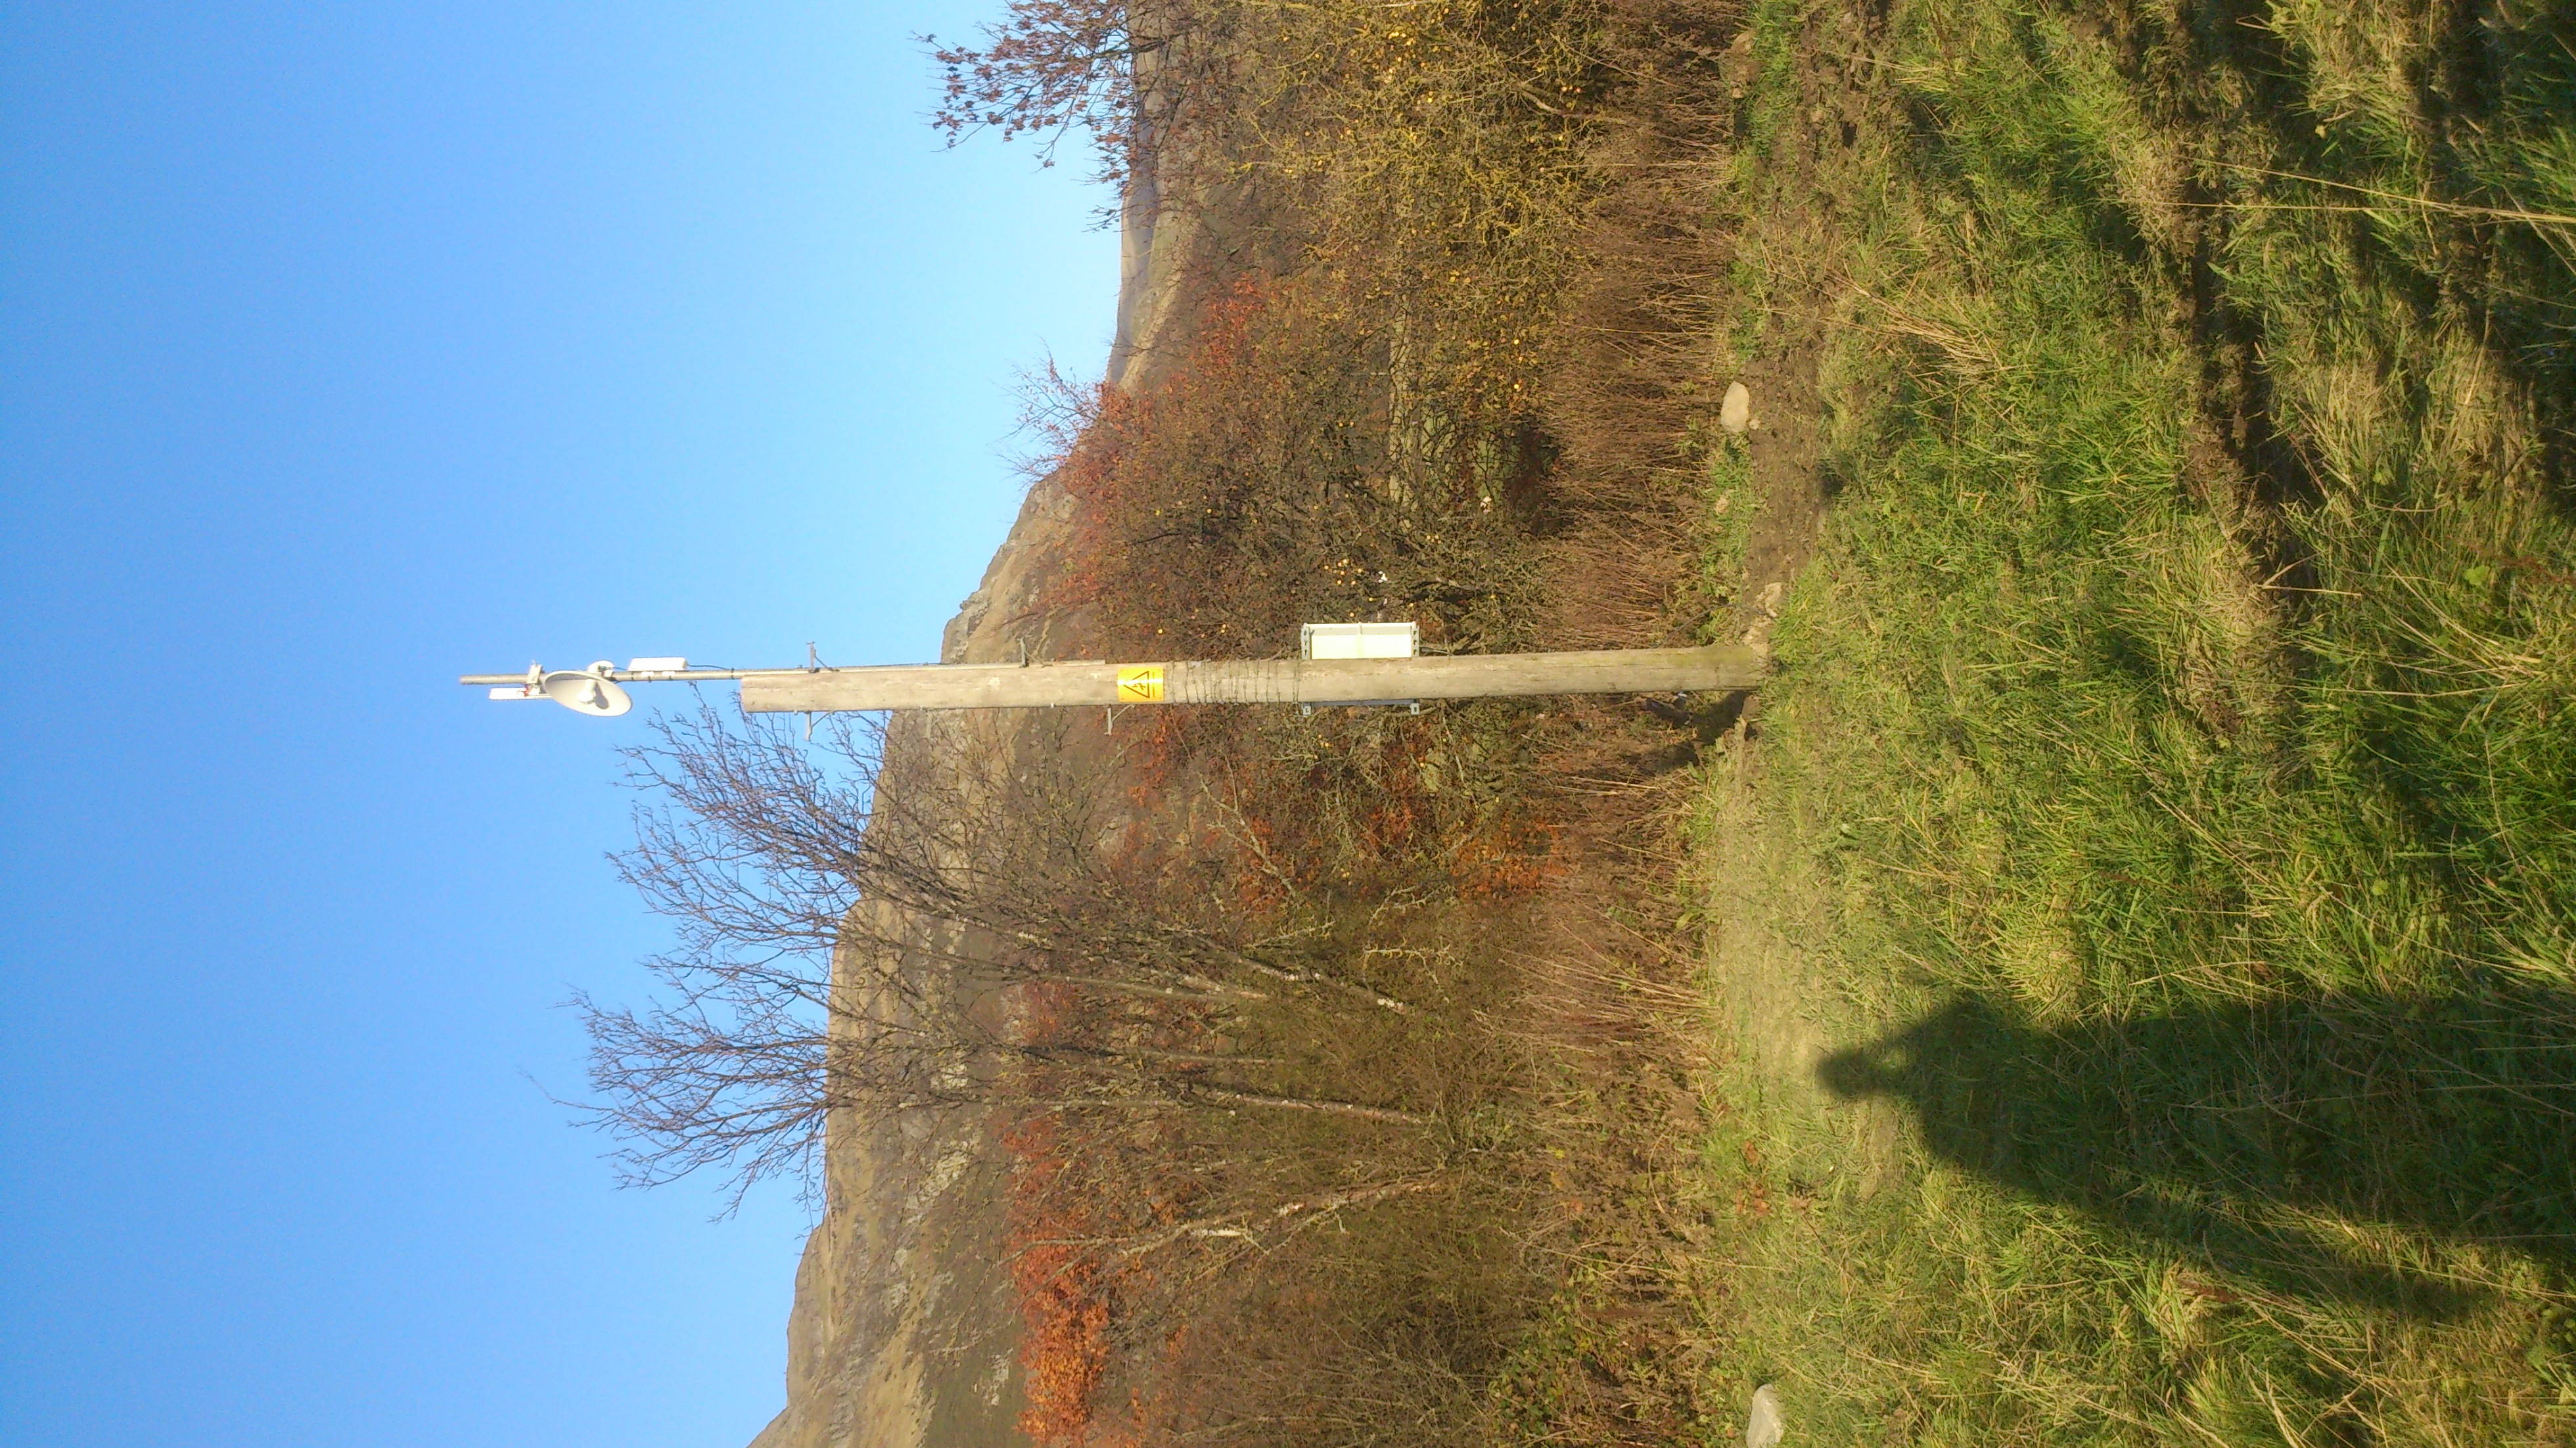
\includegraphics[width=1.1\paperwidth,angle=270]{blairmains}
%     };
%   \end{tikzpicture}
% \end{frame}
\begin{frame}
  \begin{tikzpicture}[overlay]
    \node at (5.5, -0.5) {%
      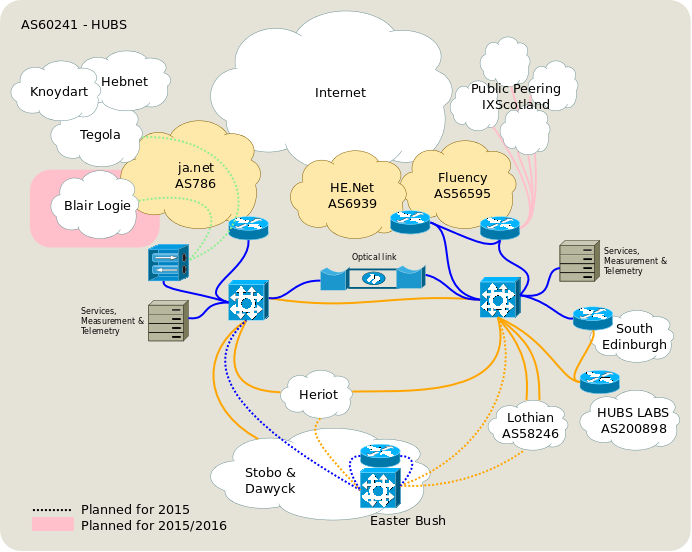
\includegraphics[width=0.8\paperwidth]{hubs-mar2015.png}
    };
  \end{tikzpicture}
\end{frame}
\begin{frame}
  \begin{center}
    \begin{tikzpicture}[overlay]
      \node at (0, -0.5) {%
        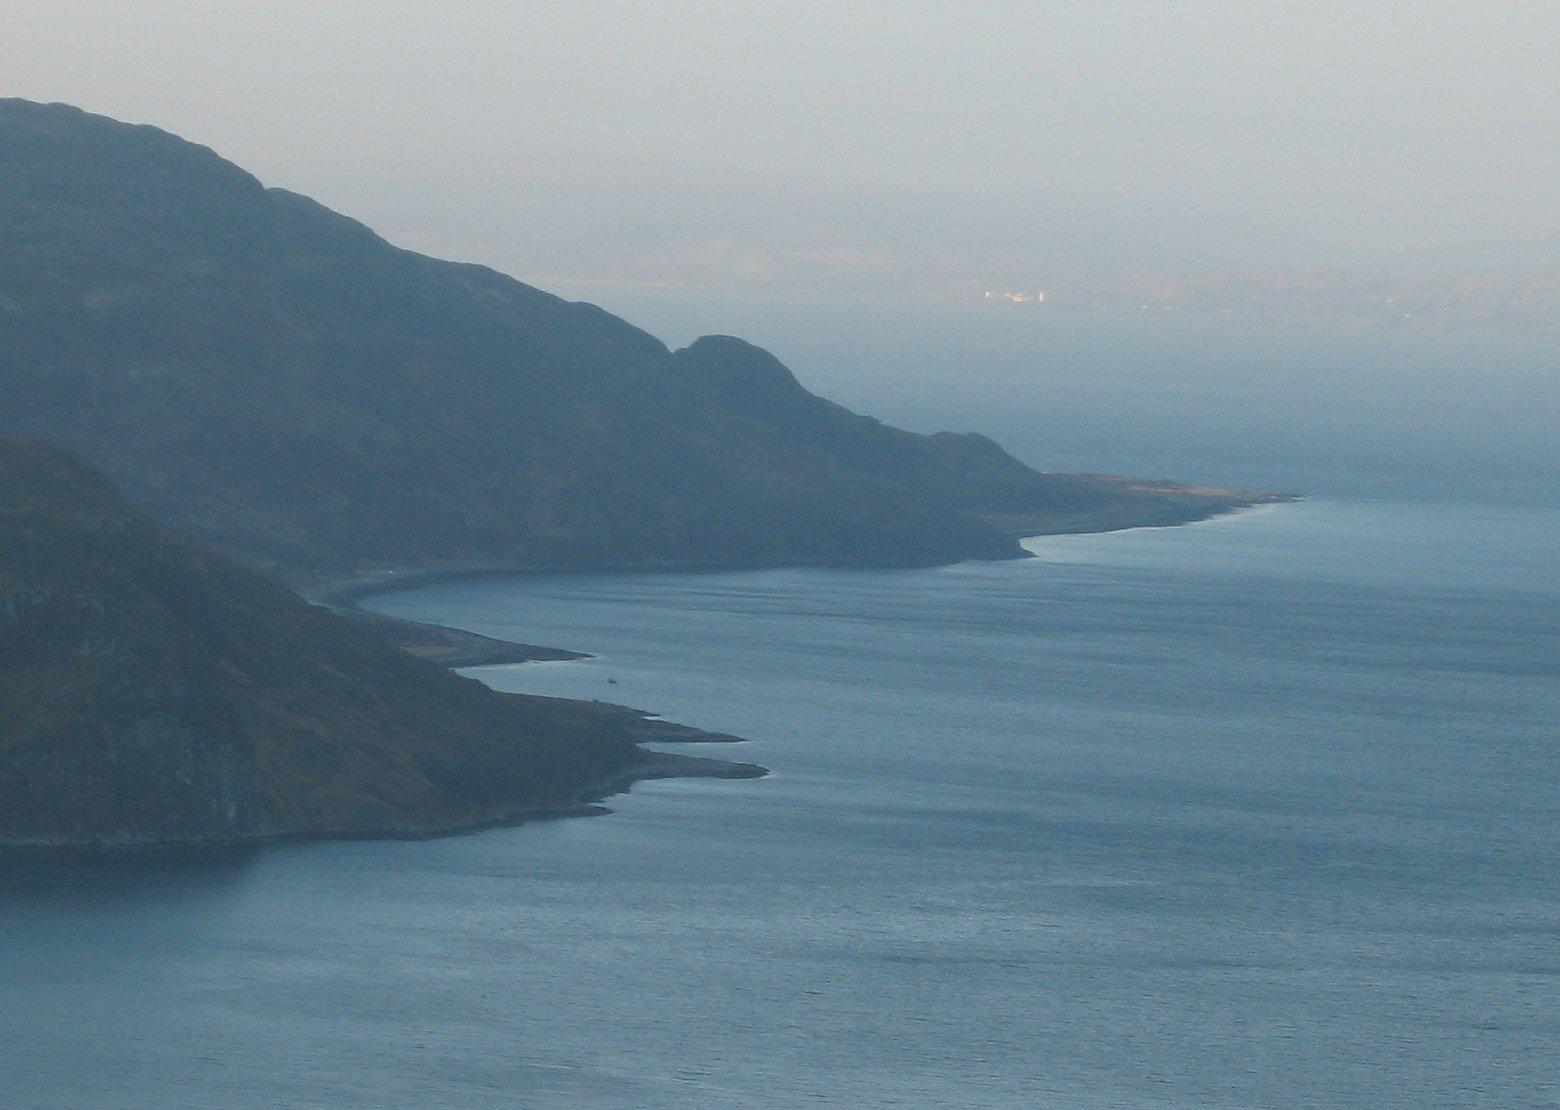
\includegraphics[height=1.1\paperheight]{scenery.jpg}
      };%
      \node at (4,3) {\Huge \color{hubsblue} Thank you};
      \node at (0,-4) {\Large \color{hubsblue}\url{http://www.tegola.org.uk/}};
      \node at (0,-4.5) {\Large \color{hubsblue}\url{http://www.hubs.net.uk/}};
    \end{tikzpicture}
  \end{center}
\end{frame}    

\end{document}
